\documentclass[FIPLY_base.tex]{subfiles}

\author{Andreas Denkmayr}
\date{25. Februar 2016}

\begin{document}
\subsection{Advertising mit AdMob}
Mit dem Schalten von Werbung steht eine weitere Einkommensquelle von Apps zur Verfügung.\newline
Es gibt mehrere Dienste die das Schalten von Werbungen unterstützen. \newline
Google AdMob ist der populärste dieser Dienste und wird von Google empfohlen. \newline
Beim Nachforschen und beim Erstellen der Werbungen wurde die Dokumentation zu diesen auf der Google Developers Webseite [\citetitle{gdAdMob} \cite{gdAdMob}] verwendet.
\ \\
\begin{figure}[h]
	\begin{subfigure}[b]{0.3\textwidth}
	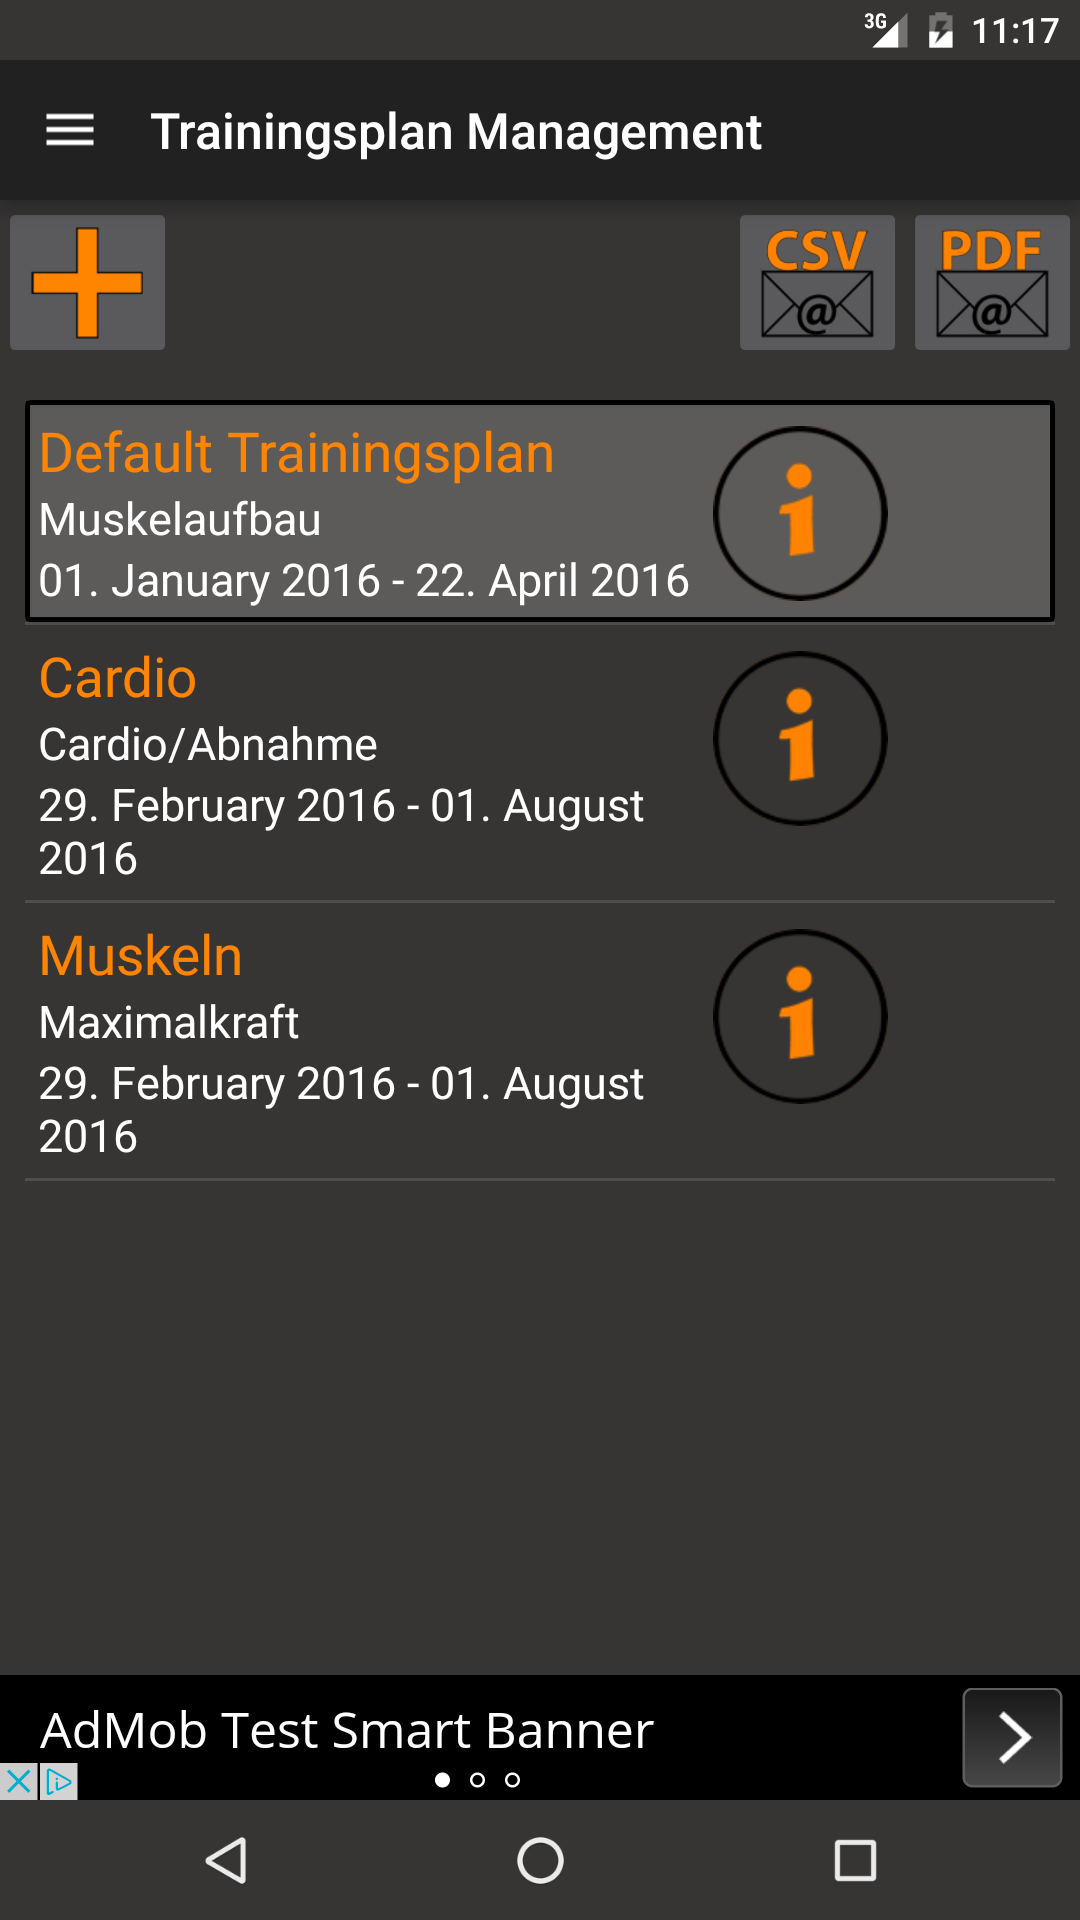
\includegraphics[scale=0.15]{img/adsBanner}
	\end{subfigure}
	\hfil
	\begin{subfigure}[b]{0.3\textwidth}
	
\includegraphics[scale=0.15]{img/adsInterstitial}
	\end{subfigure}
	\caption{Links ist ein Beispiel für eine Banner Ad zu sehen. \newline Rechts sieht man ein Beispiel für ein Interstitial.}
\end{figure}

\newpage
\subsubsection{Banner Ads}
Beim Erstellen der Banner wurde die Dokumentation zu diesen auf der Google Developers Webseite [\citetitle{gdBanner} \cite{gdBanner}] verwendet. \newline 
Banner Ads nehmen einen kleinen Teil des Bildschirms ein. Diese werden meistens in einem Layout File erstellt und dann in einer Activity oder in einem Fragment geladen. Der User kann durch einen Klick auf den Banner auf die beworbene Webseite weitergeleitet werden.
\ \\
\begin{lstlisting}
<com.google.android.gms.ads.AdView
    android:id="@+id/planAdView"
    android:layout_width="match_parent"
    android:layout_height="wrap_content"
    android:layout_centerHorizontal="true"
    android:layout_alignParentBottom="true"
    ads:adSize="SMART_BANNER"
    ads:adUnitId="ca-app-pub-3940256099942544/1033173712"
    ></com.google.android.gms.ads.AdView>
\end{lstlisting}
Hier wird ein Banner in einem xml layout file definiert. Dieses Banner befindet sich am Boden der App und überspannt die gesamte Breite des Bildschirms.
Die oben eingetragene AdUnitId liefert uns TestAds und dient zum testen.
\ \\
\begin{lstlisting}
int gender = AdRequest.GENDER_MALE;

AdView mAdView = (AdView) getActivity()
        .findViewById(R.id.planAdView);
AdRequest adRequest = new AdRequest.Builder()
        .addTestDevice(AdRequest.DEVICE_ID_EMULATOR)
        .setGender(gender)
        .build();
mAdView.loadAd(adRequest);
\end{lstlisting}
Dieser Code beinhaltet das Anfordern einer Werbung und anschließend wird diese Werbung direkt geladen.
Das Banner wird erst dann sichtbar wenn eine Werbung geladen wurde.
Die angeforderte Werbung kann durch Daten wie Geschlecht, Geburtstag oder Position präziser auf den Benutzer abgestimmt werden.
Diese Abstimmung erfolgt durch die Methoden .setGender(), .setLocation() und .setBirthday().	

\newpage
\subsubsection{Interstitial Ads}
Beim Erstellen der Interstitials wurde die Dokumentation zu diesen auf der Google Developers Webseite [\citetitle{gdInterstitials} \cite{gdInterstitials}] verwendet. \newline 
Interstitial Ads bedecken den gesamten Bildschirm. 
Dabei wird ein InterstitialAd Objekt mit einer einzigartigen Id erstellt. Später wird eine Werbung angefordert und sobald diese geladen ist wird sie angezeigt. Der Benutzer erhält die Entscheidung die Anzeige zu schließen oder dem Link der Werbung zu folgen. Deshalb eignen sich Interstitials für Apps die gelegentlich zwischen mehreren Bildschirmen wechseln.
Bei diesen Werbungen ist zu beachten, dass die App im Hintergrund weiterläuft also sollten laute Tonwiedergaben und ressourcenintensive Benutzerinteraktionen pausiert werden. Zusätzlich ist es möglich diese Interstitials in einem bestimmten Zeitintervall einzublenden.
\ \\
\begin{lstlisting}
mInterstitialAd = new InterstitialAd(this);
mInterstitialAd.
       		setAdUnitId("ca-app-pub-3940256099942544/1033173712");
requestNewInterstitial();
\end{lstlisting}
Hier wird eine Interstitial angelgegt und anschließend wird eine Werbung für das Interstitial angefordert. 
Die oben eingetragene AdUnitId liefert uns TestAds und dient zum testen.
\ \\
\begin{lstlisting}
public void requestNewInterstitial() {
        int gender = AdRequest.GENDER_MALE;
        
        AdRequest adRequest = new AdRequest.Builder()
                .addTestDevice(AdRequest.DEVICE_ID_EMULATOR)
                .setGender(gender)
                .build();
        mInterstitialAd.loadAd(adRequest);
    }
\end{lstlisting}
Mit diesem Code wird eine neues Interstitial angefordert. Die angeforderte Werbung kann durch Daten wie Geschlecht, Geburtstag oder Position präziser auf den Benutzer abgestimmt werden.
Diese Abstimmung erfolgt durch die Methoden .setGender(), .setLocation() und .setBirthday().	
\ \\
\begin{lstlisting}
if(mInterstitialAd.isLoaded()) 
    mInterstitialAd.show();
\end{lstlisting}
Ist die Werbung geladen kann sie angezeigt werden.\newline
Ebenso sind zahlreiche AdListener vorhanden die ermöglichen das Verhalten nach einer Interaktion mit der Werbung zu verwalten.
Deshalb liegt es nahe die nächste Werbung gleich im onAdClosed() eines AdListeners anzufordern.





\begin{lstlisting}
\end{lstlisting}
\end{document}
